\section{Address Resolution Protocol (ARP)}

ARP es un protocolo de capa 2 (capa de enlace), que trabaja con Ethernet y otros protocolos de capa 2 para ayudar a IP. Es un protocolo \textbf{helper} de IP. Su función principal es mapear direcciones lógicas a físicas (mapear dirección IP a dirección MAC). Utiliza auto-aprendizaje, no requiere de configuración (es dinámico). Es encapsulado dentro de una trama Ethernet.

\begin{nota}{\textbf{Recordar} \newline}
    ARP funciona dentro de un dominio de \emph{broadcast}, no permite determinar la dirección MAC de un dispositivo en otra red.
\end{nota}

Cada nodo tiene una tabla ARP en memoria que contiene la relación entre una IP y una MAC. 

\subsection{Funcionamiento de ARP}

Supongamos que PC-A y PC-B están en un mismo dominio de broadcast. Si A le quiere enviar un mensaje a B, debe primero conocer su dirección MAC. Por la IP A sabe que B está en su misma red, entonces envía un \textbf{ARP Request} a la MAC de broadcast (ff:ff:...:ff) con la IP a la que debe enviarle el mensaje.

\begin{figure}[htbp]
    \centering
    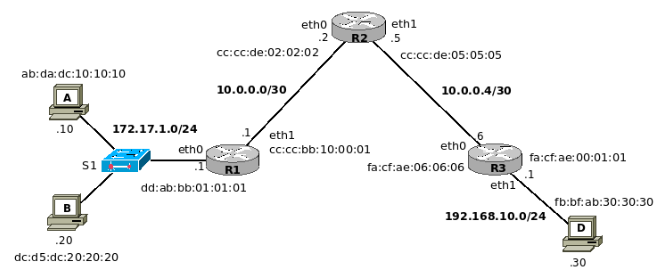
\includegraphics[width=0.7\textwidth]{capitulos/arp/imagenes/topologia-ejemplo.png}
    \caption{Topología del ejemplo}
    \label{fig:ejemplo-arp}
\end{figure}

El nodo que tenga la IP destino asignada, procesará y responderá al ARP Request con un \textbf{ARP Reply} de tipo unicast. Una vez respondido, A ya puede enviarle mensajes a B por tener su dirección física. 

Ahora supongamos que PC-A le quiere enviar un mensaje a PC-D, que está en \textbf{otra red}. Para llegar a D, A debe encontrar la MAC de su \emph{default gateway}. El procedimiento es el mismo que para el caso anterior: ARP Request a la dirección de broadcast y el router de gateway responde con un ARP Reply.

Ahora, A envía el mensaje \textbf{Echo Request} con la interfaz del router como MAC destino. Cuando llega el mensaje, el router rutea el paquete y lo pasa a la capa inferior para forwardearlo por la interface que corresponda. El paquete puede ser enviado a otro router o al destino final, y si el router no conoce la MAC destino debe volver a ejecutar ARP para cambiar los campos de la trama Ethernet. 